\begin{figure*}[!ht]
\centering
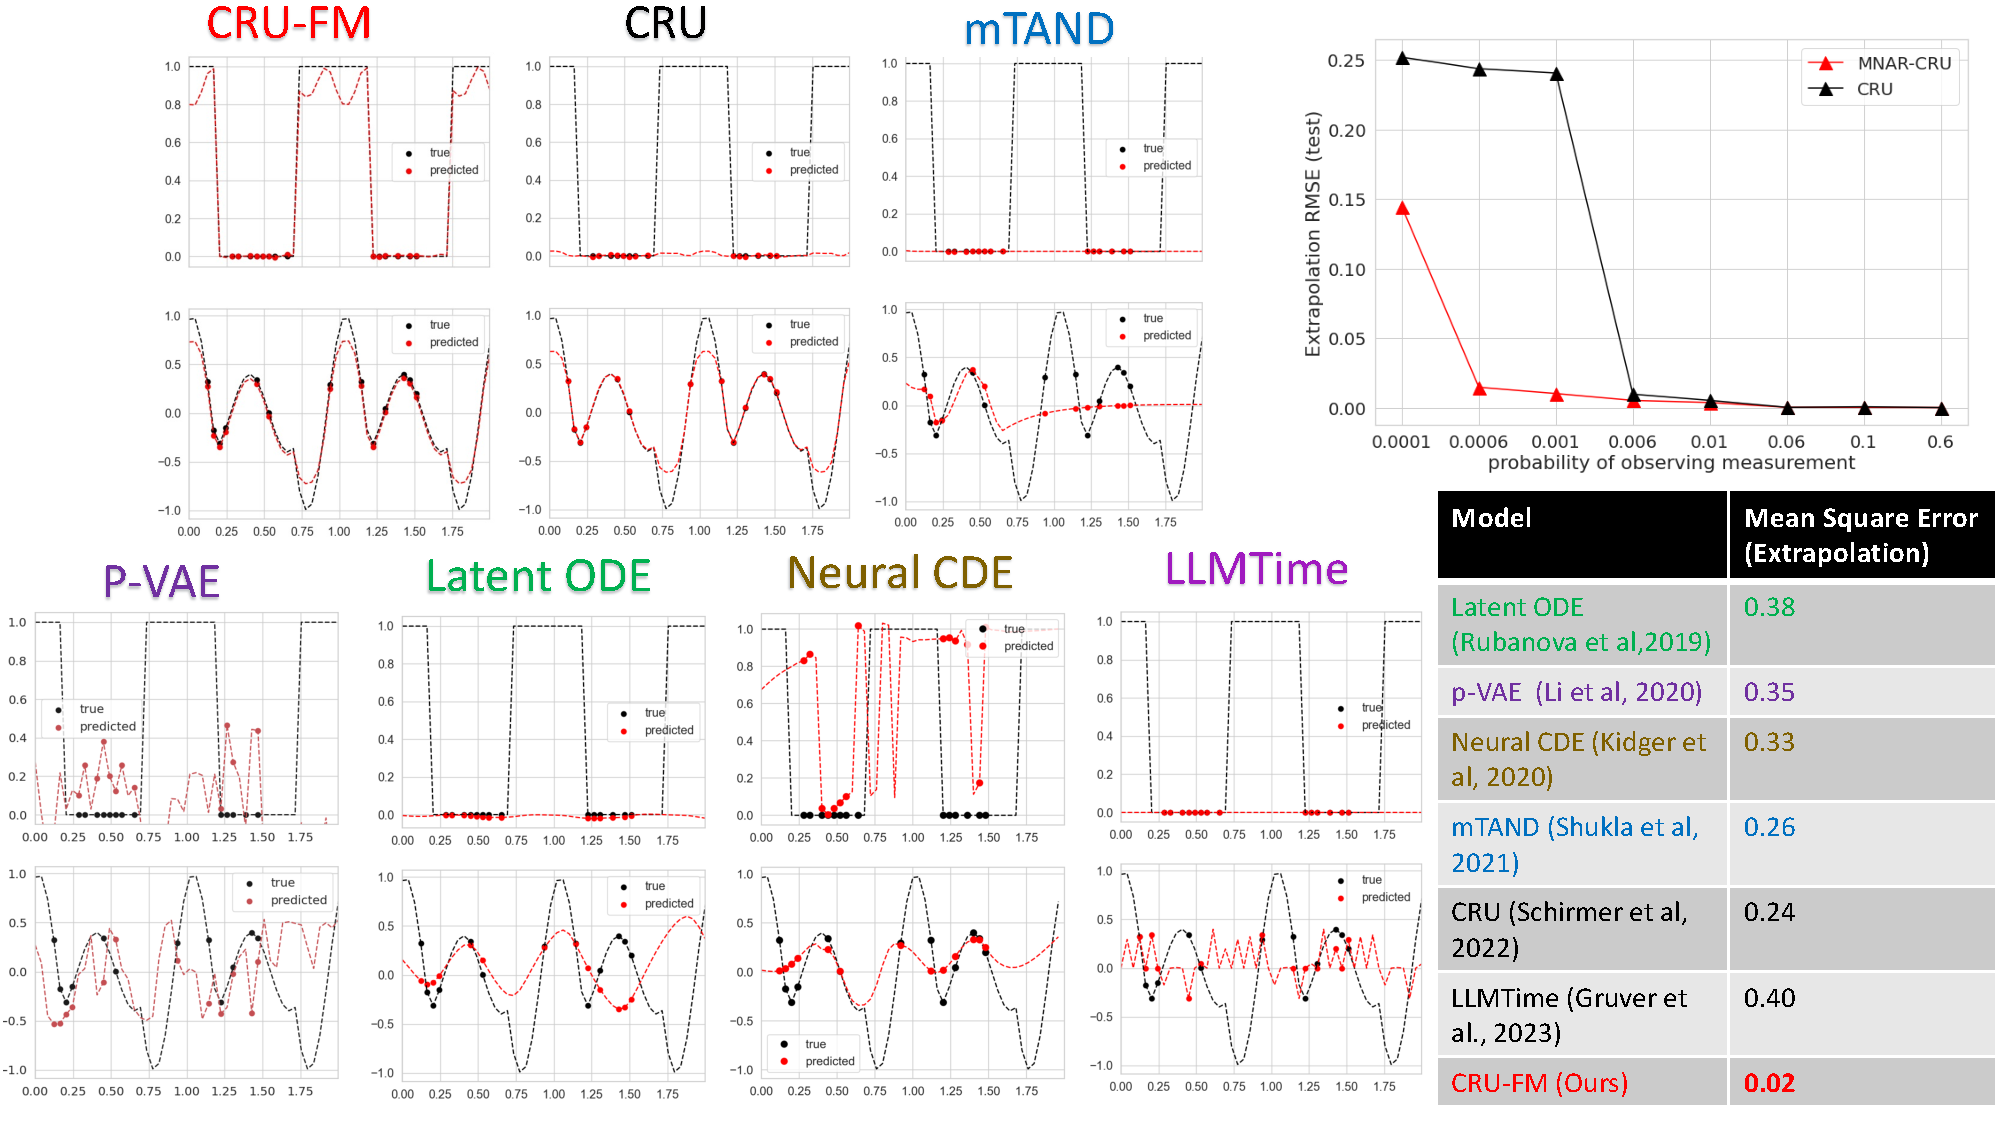
\includegraphics[width=1.0\textwidth]{content/chapters/irregular_time_series_data_driven_missingness/figures/toydata_extrapolation_improved.pdf}
\caption[Synthetic task results comparing CRU-FM to competitors]{Synthetic task results comparing CRU-FM to competitors.
\emph{Left:} Visuals of reconstruction ($t \in (0, 1.5)$) and extrapolation ($t \in (1.5, 2)$) for the \emph{same} 2-channel test sequence when missingness is data-dependent ($p_{\text{S}} {=} 0.0006$).
Black (red) lines indicate true (reconstructed) values. To fairly compare models, we evaluate each one's most likely prediction $\hat{x}_{t}$ (mode of the predictive distribution). 
For example, for our CRU-FM we set $\hat{x}_{t} = h_{t}$ (via Eq.~\eqref{eq:mnar_cru_model}).
This choice eliminates extraneous randomness needed to sample from a predictive distribution.  \emph{Bottom Right:}
Extrapolation results on the synthetic task sequences comparing MNAR-CRU, CRU, MTAND and p-VAE. The black/red dots are the observed/predicted values at each irregularly sampled time point. The black/red line is the true/reconstructed sequence. Each model is trained until $t=1.5$ and the extrapolated from $t=1.5$ to $t=2$. MNAR-CRU generates sequences that are closer to the ground-truth and also achieves the least mean squared error on the extrapolation task. We attribute this improved performance of the MNAR-CRU to the model's ability to learn the true missingness probability in each sequence. \textit{Top right :} We examine how extrapolation error changes as the probability of observing a measurement (denoted as $p_{obs}$) outside the (-0.4, 0.4) bounds changes. As $p_{obs}$ increases (MNAR assumption relaxes), as expected the CRU and MNAR-CRU perform similarly. For low values $p_{obs} \leq 0.006$, MNAR-CRU’s better-specified missingness model notably improves extrapolation (via a joint model of $x_t$ and $s_t$).
}%endcaption
\label{fig:models_generated_seq}
\end{figure*}